\section{Navigation Screens}

Until a user approaches and interacts with the display \textbf{security tips} are getting dynamically fetched by the LLM and shown on the screen.
These messages, shown in Figure 2.1, are designed to catch user's attention and encourage them to engage with our \textbf{SeQG} and learn more about \textbf{cybersecurity}.
On touch interaction the user gets navigated to the \textbf{mode selection} screen.

\begin{figure}[H]
    \centering
    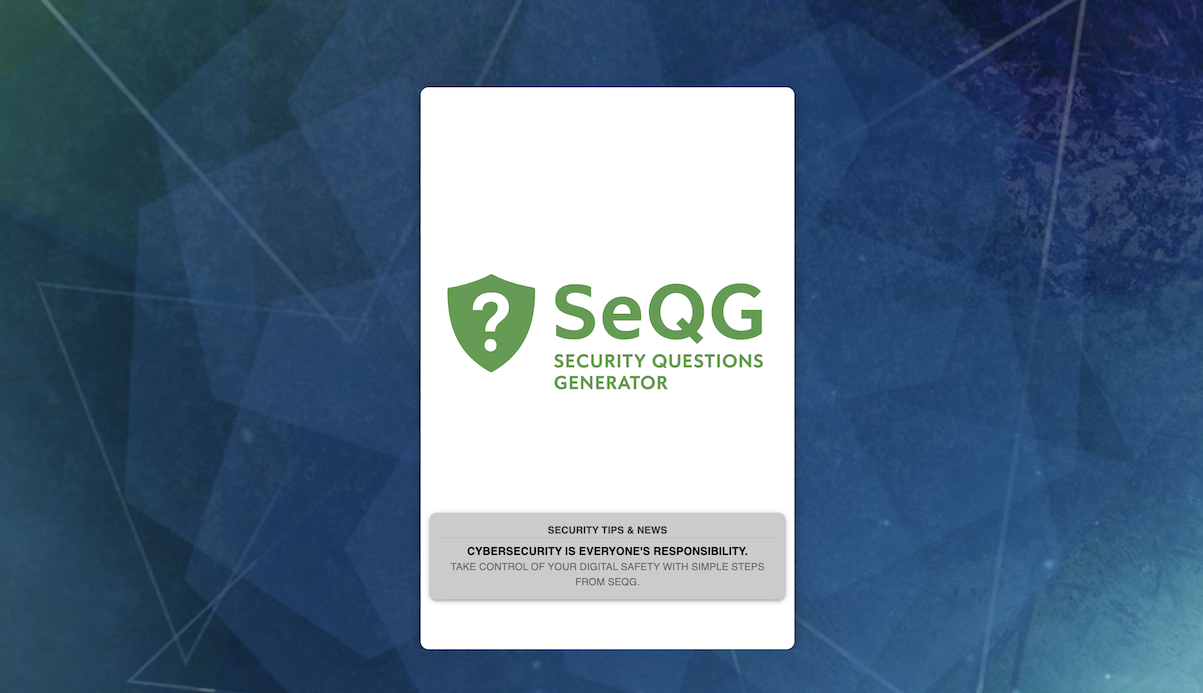
\includegraphics[width=0.8\textwidth]{images/MainScreen1.png}
    \caption{Main Screen}
\end{figure}

The \textbf{mode selection} allows the user to choose between one of \textbf{two mode characters}, each accompanied with a short explanation of their mode representation as to be seen in Figure 2.3. 
The characters rotate on swipe or by pressing the button below. 
To select a mode the user must rotate to the character and click the Enter Button on the bottom of the page. 
Afterwards he gets navigated to the according Session login.

\begin{figure}[H]
    \centering
    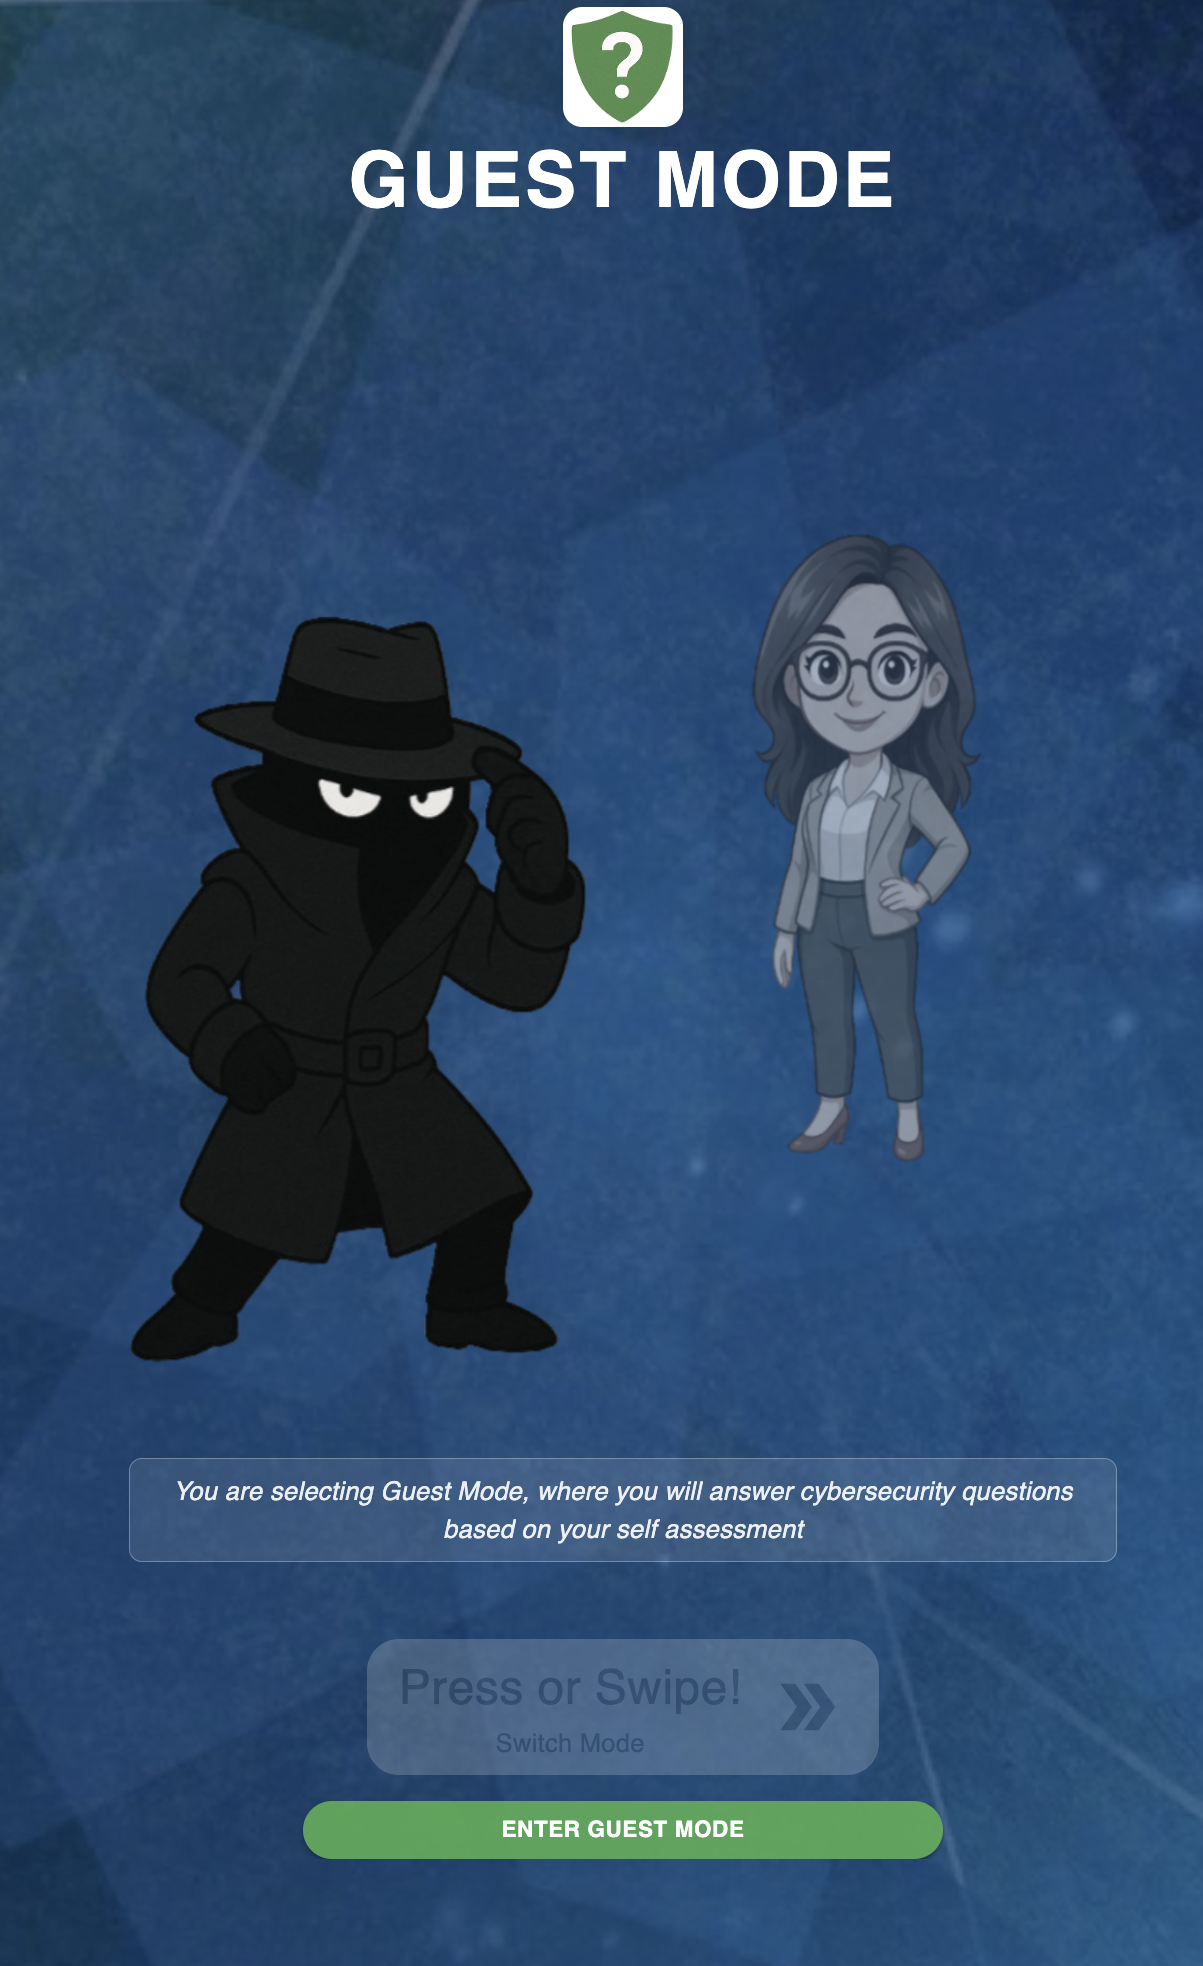
\includegraphics[width=0.4\textwidth]{images/MainScreenCharacter1.png}
    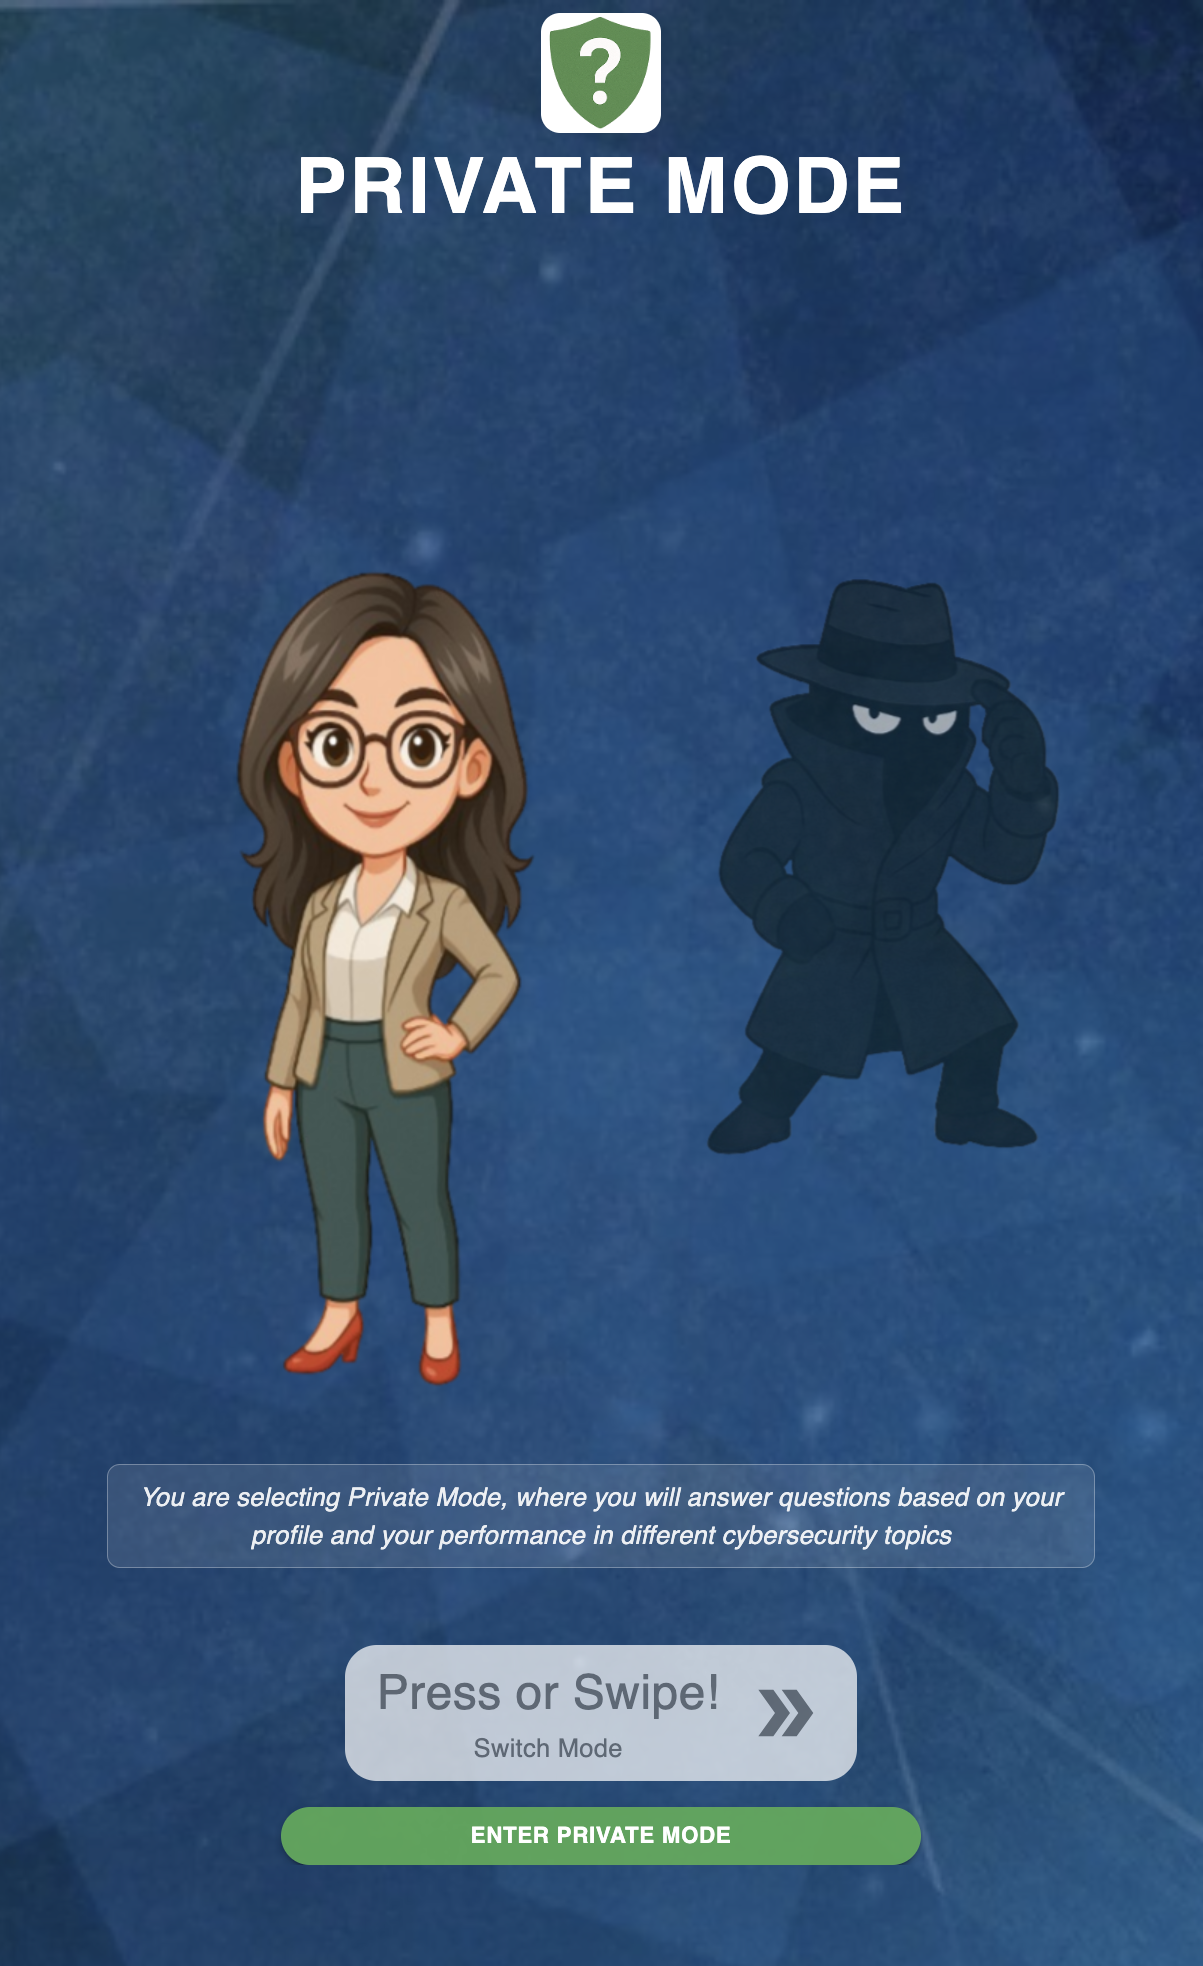
\includegraphics[width=0.4\textwidth]{images/MainScreenCharacter2.png}
    \caption{Characters for Mode selection}
\end{figure}
